\documentclass{llncs}

\usepackage{amsmath}
\usepackage{amssymb}
\usepackage{graphicx}
\usepackage{url}
\usepackage{boxedminipage}
\usepackage{oz}

\setcounter{tocdepth}{3}
\def\keywordname{{\textbf{Keyword:}}}
\newcommand{\keywords}[1]{\par\addvspace\baselineskip
\noindent\keywordname\enspace\ignorespaces#1}

\begin{document}

\mainmatter  % start of an individual contribution

\title{PODD: An Ontology-driven Data Repository for Collaborative Phenomics Research}

\author{Yuan-Fang Li \and Gavin Kennedy \and Faith Davies \and Jane Hunter}

\institute{School of ITEE, The University of Queensland
\email{\{uqyli4,g.kennedy1,f.davies,j.hunter1\}@uq.edu.au}}

\maketitle

\begin{abstract}
Phenomics, the systematic study of phenotypes, is an emerging field
of research in biology. It complements genomics, the study of
genotypes, and is becoming an increasingly critical tool to
understand phenomena such as plant morphology and human diseases.
Phenomics studies make use of both high- and low-throughput imaging
and measurement devices to capture data, which are subsequently used
for analysis. As a result, high volumes of data are generated on a
regular basis, making storage, management, annotation and
distribution a challenging task. Sufficient contextual information,
the metadata, must also be maintained to facilitate the
dissemination of these data. The challenge is further complicated by
the need to support emerging technologies and processes in phenomics
research. This paper describes our effort in designing and
developing an ontology-driven, open, extensible data repository to
support collaborative phenomics research in Australia.

\keywords{OWL, ontology, repository, phenomics, data management}
\end{abstract}

\section{Introduction}\label{sec:intro}
An organism's phenotype is an observable or quantifiable trait of
the organism as a consequence of its genetic makeup combined with
its developmental stage, environment and disease conditions.
Phenomics is the systematic and comprehensive study of an organism's
phenotype and is determined through a combination of high-throughput
and high-resolution imaging- and measurement-based analysis
platforms. Phenomics research, together with genomics research,
represents a holistic approach to biological
study~\cite{dhoule09,Sauer200458,nevo01}.

Unlike genomics, phenomics research emphasizes physical, observable
traits of the subject under study. Like genomics, vast amounts of
data are produced by imaging and measurement platforms and analysis
tools. The storage, management, analysis and publication of these
data is a challenging problem.

Specifically, there are three key challenges for data management in
phenomics research.
\begin{itemize}
\item The ability to provide a data management service that can
manage large quantities of heterogeneous data in multiple formats
(text, image, video) and not be constrained to a finite set of
imaging and measurement platforms and data formats.

\item The ability to support metadata-related services to
provide context and structure for data within the data management
service to facilitate effective search, query and dissemination.

\item The ability to accommodate evolving and emerging technologies
and processes as phenomics is still a rapidly developing field of
research.
\end{itemize}

The Phenomics Ontology Driven Data (PODD)
repository\footnote{\url{http://www.itee.uq.edu.au/~eresearch/projects/podd/}}
is being developed to meet the above challenges facing the
Australian phenomics research community, aiming at providing
efficient and flexible repository functionalities for large-scale
phenomics data. An important goal of PODD is to provide a mechanism
for maintaining structured and precise \emph{metadata} around the
raw data so that they can be distributed and published in a reusable
fashion.

Differences in research project reporting, organisms under study,
research objectives, research methodologies and imaging and
measurement platforms may result in differences in the \emph{models}
of data. In order to accommodate as wide a variety of biological
research activities as possible, we have constructed the domain
model using OWL~\cite{hoph03a} ontologies, instead of the
traditional UML class diagrams and database schemas. The OWL domain
model is at the core of the PODD repository as it drives the
creation, storage, validation, query and search of data and
metadata. In contrast to traditional data repositories that use
database schemas as the underlying model, the employment of OWL
ontologies as the domain model makes PODD highly extensible.

In this paper, we present our work in addressing the above
challenges and highlight the OWL-based modeling approach we take.
The rest of the paper is organized as follows. In
Section~\ref{sec:overview} we present some related work and give a
brief overview of PODD and relevant technical background.
Section~\ref{sec:design} presents the high-level design of the
repository. In Section~\ref{sec:ont}, we discuss the PODD domain
ontology in more detail and show how the ontology-based modeling
approach is used in the life cycle of domain objects. Finally,
Section~\ref{sec:conclusion} concludes the paper and identifies
future directions.

\section{Overview}\label{sec:overview}
\subsection{Related Work}
In biological research, a large number of databases have been
developed to host a variety of information such as genes
(Ensembl\footnote{\url{http://www.ensembl.org/}}), proteins
(UniProt\footnote{\url{http://www.uniprot.org/}}), scientific
publications
(PubMed\footnote{\url{http://www.ncbi.nlm.nih.gov/pubmed/}}) and
micro-array data
(GEO\footnote{\url{http://www.ncbi.nlm.nih.gov/geo/}}).

These databases are generally characterized by the fact that they
specialize in a particular kind of data (protein sequences,
publications, etc.) and the conceptual domain model is relatively
well understood and stable. As a result, the need for extensibility
and flexibility is not very high.

Phenomics is a fast growing discipline in biology and new
technologies and processes are evolving and emerging rapidly. As a
result, the domain model must be flexible enough to cater for such
changes. Currently there are a number of related domain models
available.

Functional Genomics Experiment Model (FuGe)~\cite{citeulike:1756058}
is an extensible modeling framework for high-throughput functional
genomics experiments, aiming at increasing the consistency and
efficiency of experimental data modeling for the molecular biology
research community. Centered around the concept of experiments, it
encompasses domain concepts such as protocols, samples and data.
FuGe is developed using UML from which XML Schemas and database
definitions are derived. The FuGe model covers not only
biology-specific information such as molecules, data and
investigation, it also defines commonly-used concepts such as audit,
reference and measurement.

Extensions in FuGe are defined using inheritance of UML classes. We
feel that the extensibility we require is not met by FuGe as any
addition of new concepts would require the development of new
database schemas and code. Moreover, the concrete objects reside in
relational databases, making subsequent integration and
dissemination more difficult.

The Ontology for Biomedical Investigations
(OBI)\footnote{\url{http://obi-ontology.org/}} is an on-going effort
of developing an integrative ontology for biological and clinical
investigations. It takes a top-down approach by reusing high-level,
abstract concepts from other ontologies. It includes 2,600+
OWL~\cite{hoph03a} classes and 10,000+ axioms (in the import closure
of the OBI ontology). Although OBI is very comprehensive, its size
and complexity makes reasoning and querying of OBI-based ontologies
and RDF graphs computationally expensive and time consuming.

\subsection{The PODD Repository}
Under the National Collaborative Research Infrastructure Strategy
(NCRIS), the Australian Government has funded two major phenomics
initiatives: The Australian Plant Phenomics Facility (APPF),
specializing in phenotyping crop and model plant species; and the
Australian Phenomics Network (APN), which specializes in the
phenotyping of mouse models. Both facilities have common
requirements to gather and annotate data from both high- and
low-throughput phenotyping devices. The scale of measurement can be
from the micro or cellular level, through the level of a single
organism, and up to (in the case of the APPF) the macro or field
level.

An organism's phenotype, observable and quantifiable traits, is
often the product of the organism's genetic makeup, its development
stage, disease conditions and its environment. Any measurement made
against an organism needs to be recorded in the context of these
other data. The opportunity exists to create a repository to record
the data, its contextual data (metadata) and data classifiers in the
form of ontological or structured vocabulary terms. The structured
nature of this repository would support manual and autonomous data
discovery as well as provide the infrastructure for data based
collaborations with domestic and international research
institutions. Currently there are no such integrated systems
available to the two facilities.

The National eResearch Architecture Taskforce (NeAT) Australia
initiated the PODD project to fill this gap. In PODD, we have
engaged in the design and development of the Phenomics Ontology
Driven Data (PODD) repository. The goal of PODD is to capture,
manage, annotate and distribute the data generated by phenotyping
platforms. It supports both Australian and international biological
research communities by providing repository and data publication
services.

\subsection{The OWL Ontology Language}
The Web Ontology Language (OWL)~\cite{hoph03a} is one of the
cornerstone languages in the Semantic Web technology stack. Based on
description logics~\cite{DBLP:conf/dlog/McGuinness03}, OWL DL (a sub
species of OWL) defines a precise and unambiguous semantics, which
is carefully crafted so that it is very expressive yet core
reasoning tasks can be fully automated.

Information in OWL, as in RDF~\cite{rdfprimer04}, is modeled in
triples: $\langle subject, predicate,\allowbreak object\rangle$,
where $subject$ is the entity of interest, $predicate$ represents a
particular characteristic/property of the entity and $object$ is the
actual value of that property. \emph{Class}es are first-class
citizens in OWL. They represent abstract concepts in a particular
domain. Concrete objects are represented by OWL \emph{individual}s.
OWL \emph{predicate}s are used to relate OWL entities (classes,
individuals, predicates) to their attributes or other entities.

\vspace{-16pt}
\begin{figure}[htb]
\scriptsize
\hspace{-28pt}
\begin{minipage}[t]{0.6\textwidth}
\begin{syntax}
\mathcal{C} &::= &C                              & Class name\\
            & |  &\top                           & Top class\\
            & |  &\bot                           & Bottom class\\
            & |  &\mathcal{C} \sqcup \mathcal{C} & Class union\\
            & |  &\mathcal{C} \sqcap \mathcal{C} & Class intersection\\
            & |  &\lnot \mathcal{C}              & Class negation\\
            & |  &\forall P.\mathcal{C}          & Universal quantification\\
            & |  &\exists P.\mathcal{C}          & Existential quantification\\
            & |  &P\colon o                      & Value restriction\\
            & |  &\geq n~ P                      & At least number restriction\\
            & |  &\leq n~ P                      & At most number restriction\\
            & |  &\{a_1, \cdots, a_n\}           & Enumeration
\end{syntax}
\vspace{-16pt}
\caption{OWL expressions}\label{fig:owl-des}
\end{minipage}
%
\hspace{-12pt}
\begin{minipage}[t]{0.45\textwidth}
\begin{syntax}
\mathcal{AX} &::=& C \sqsubseteq \mathcal{C}                & Class subsumption\\
             & | & C = \mathcal{C}                          & Class equivalence\\
             & | & C \sqcap \mathcal{C} = \bot              & Class disjointness\\
             & | & P \sqsubseteq P                          & Property subsumption\\
             & | & P = P                                    & Property equivalence\\
             & | & \geq 1~ P\sqsubseteq \mathcal{C}         & Property domain\\
             & | & \top \sqsubseteq \forall P.\mathcal{C}   & Property range\\
             & | & \top \sqsubseteq \leq 1~ P               & Functional property\\
             & | & P = ({}^- P)                             & Inverse property
\end{syntax}
\vspace{+20pt} \centering\caption{OWL class and predicate
axioms}\label{fig:owl-axm}
\end{minipage}
\end{figure}

\vspace{-12pt}
\emph{Class descriptions} can be used to construct (anonymous)
complex class expressions from existing ones, as shown in
Figure~\ref{fig:owl-des}. $\mathcal{C}$ represents (possible
complex) class expressions; $C$ is a class name; $P$ stands for a
predicate; $n$ is a natural number and $a_i$'s are individuals.
OWL uses \emph{axioms} to place restrictions on OWL classes and
predicates. These axioms include class subsumption, equivalence,
disjointness; predicate domain, range, etc. Figure~\ref{fig:owl-axm}
shows some of the axioms.

The OWL language has been widely used in life sciences and
biotechnology~\cite{journals/bib/RuttenbergRSM09,citeulike:1882392,citeulike:212874}
as a modeling language for its expressivity and extensibility. There
is also growing tool support for tasks such as reasoning, querying
and visualization, making it a viable option for the modeling and
representation of domain concepts and objects in phenomics.

\section{High-level Design of PODD}\label{sec:design}
PODD is intended to be an open platform that allows any user to
access data that is either published or explicitly shared with them
by the data owners. Moreover, PODD has been envisioned to provide
data management services for a wide variety of research projects and
phenotyping platforms.

The key design considerations of PODD include:
\begin{itemize}
\item Data storage and management. It is estimated that several TB
of data will be generated by PODD clients per year. Hence, the
ability to efficiently manage large volumes of data is crucial.

\item Repository reusability. Data generated by a wide range of
projects and phenotyping platforms will be stored in the repository.
Hence, the domain model needs to be flexible enough to cater for the
administrative, methodological and technical differences across
projects and platforms.

\item Data persistence and identification. In order to support the
dissemination of scientific findings, data in the repository needs
to be publicly accessible after being published. Hence, a persistent
naming scheme is required.
\end{itemize}

In the development of PODD we employ a number of core technologies
to meet the above requirements.

\begin{itemize}
\item We use Fedora Commons\footnote{\url{http://www.fedora-commons.org/}}, a digital
repository for the management, storage and retrieval of domain
objects.

\item We use iRODS~\cite{irods07}, a distributed, grid-based storage
software system, for the actual storage solution of domain objects
across a virtual data fabric.

\item We incorporate the Sesame\footnote{\url{http://www.openrdf.org/}}
triple store for the storage and query of RDF triples (ontology
definitions of concrete objects).

\item We use the Lucene\footnote{\url{http://lucene.apache.org/}}
open-source search engine for the full-text index and search of repository
contents, including values in the RDF triple store.
\end{itemize}

The high-level architecture of the PODD repository can be seen in
Figure~\ref{fig:arch}.

\begin{figure}[htb]
\centering
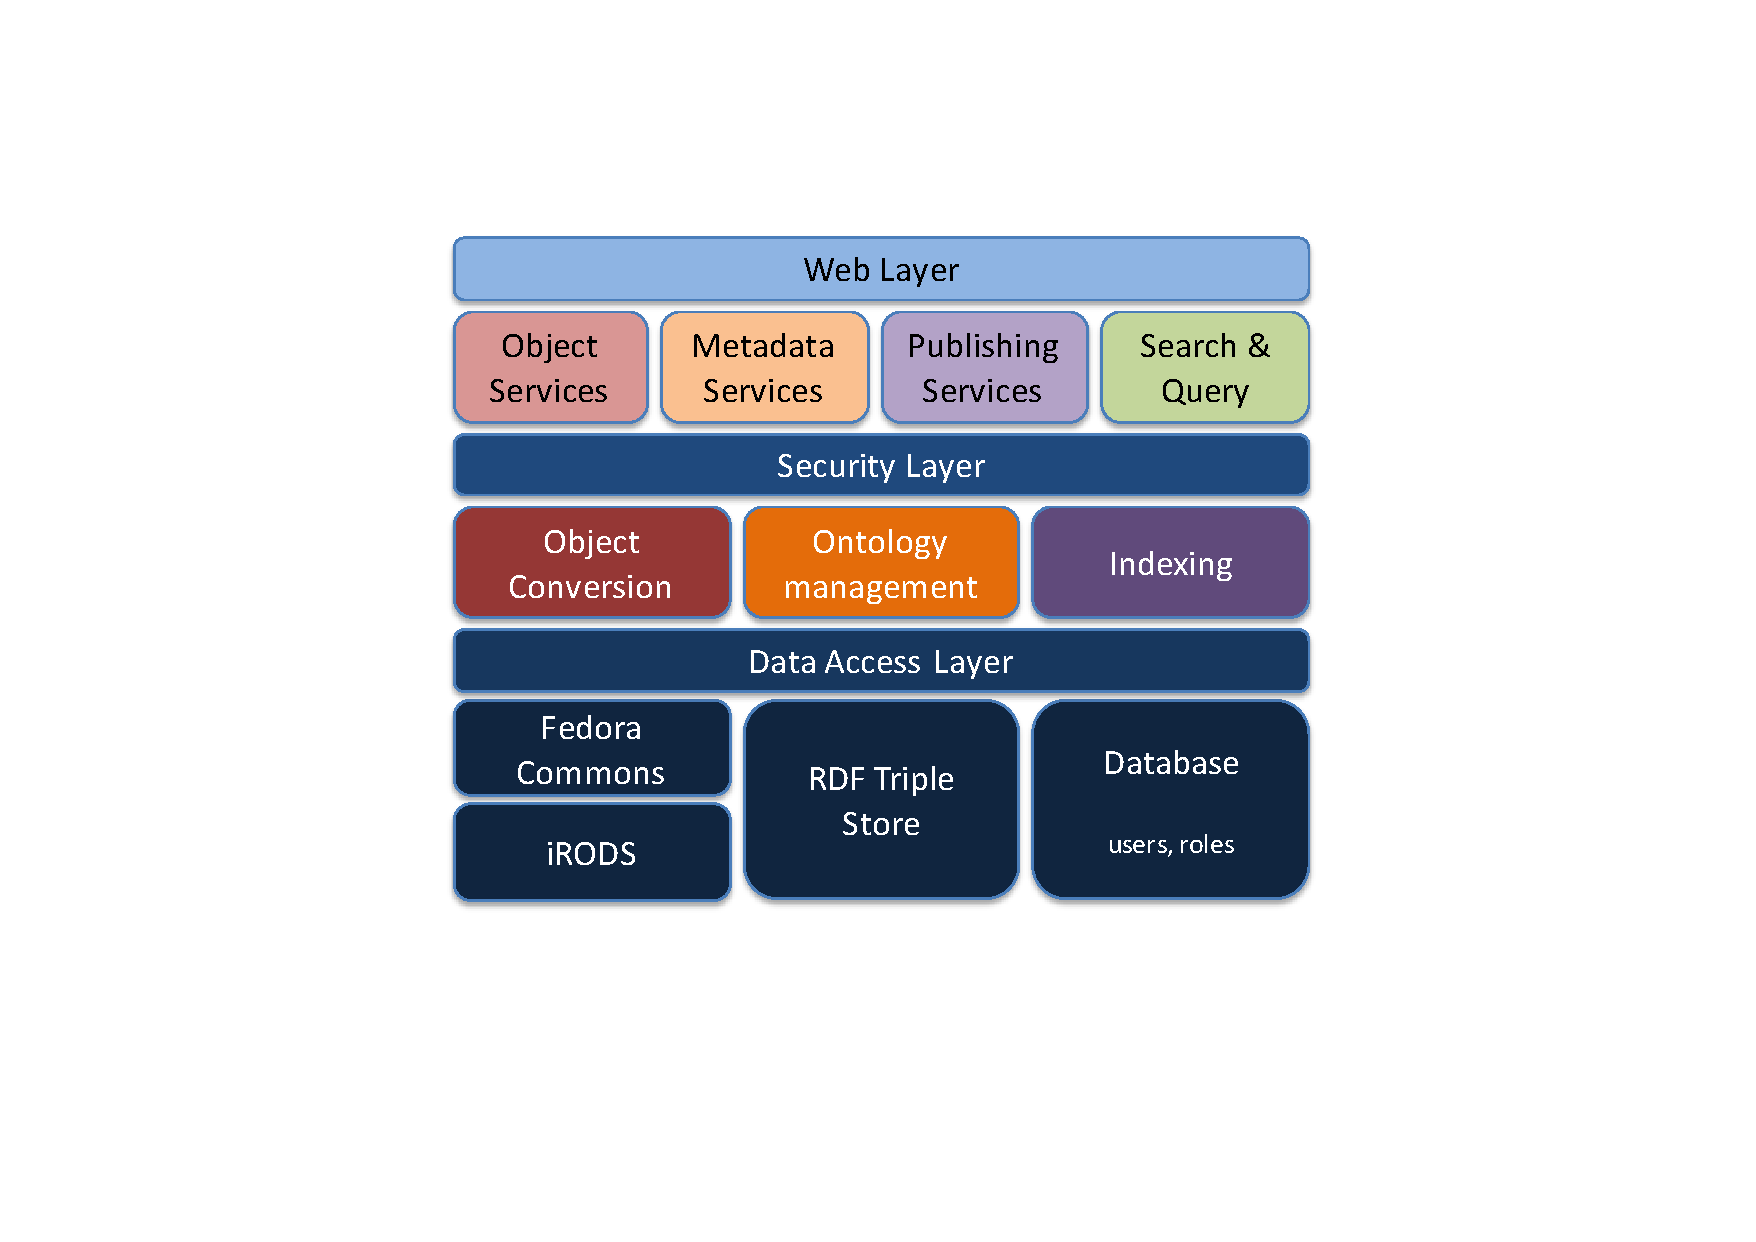
\includegraphics[trim = 45mm 50mm 45mm 40mm, clip,height=70mm]{architecture.pdf}
\vspace{-16pt} \caption{The high-level architecture of the PODD
repository.}\label{fig:arch}
\end{figure}

\section{Ontology-based Domain Modeling}\label{sec:ont}
One of the important design decisions to be made early in the
development process is the domain model. Domain modeling aims at
providing solutions for two important tasks. Firstly, efficient and
flexible data organization; and secondly, data contextualization in
the form of \emph{metadata}, so as to provide meaning for the raw
data (documents, publications, image files, etc.) to facilitate
search, query, dissemination, and so on.

As we emphasized previously, the domain model should be flexible
enough to accommodate the rapid changes and advancement of phenomics
research. Inspired by FuGe and OBI, we created our own PODD ontology
in OWL to define essential domain concepts and relations.
%To
%improve interoperability, we maintain mappings between terms in the
%PODD and OBI ontologies through annotations.

\subsection{The PODD Ontology}
As PODD is designed to support the data management tasks for
phenomics research, a number of essential domain concepts and the
relationships between these concepts need to be modeled. Domain
concepts will be modeled as OWL classes; relationships between
concepts and object attributes will be modeled as OWL object- and
datatype-predicates. Concrete objects will be modeled as OWL
individuals.

\subsubsection{The Domain Concepts} In our modeling, the top-level
concept is \textbf{\emph{Project}}, which is an administrative
concept and contains essential meta information about the research
project, such as the administering organization, principal
investigator, project membership, project status, etc.

A number of concepts may be associated with the project concept.

\begin{description}
\item[\emph{Project Plan}] describing the
current project plan at the core metadata element level.

\item[\emph{Platform}] describing any single technical
measurement platform used in the project. Technical measurement
platform means any platform for which parameters and parameter
values may be captured.

\item[\emph{Genotype}] describing the genotype of the
materials used in the investigations. Multiple genotypes are
described here and then can become fields in the instances of the
Material object.

\item[\emph{Investigation}] describing a planned process
within a project that executes some form of study design and
produces a coherent set of results. It can be considered equivalent
to an experiment.
\end{description}

The \textbf{\emph{Investigation}} concept is of central importance.
It captures the data and metadata of experiments under a project. A
number of concepts are defined to assist in the modeling of
investigations.

\begin{description}
\item[\emph{Experimental Design}] describing experimental design
components, e.g. plant layouts, sampling strategies, etc.

\item[\emph{Growth Condition}] describing growth conditions, such as
growth chambers used, environmental settings, etc.

\item[\emph{Process}] representing a planned component of an
investigation. It is a description of a series of steps taken to
achieve the objective of the investigation.

\item[\emph{Protocol}] describing a step within a process that is a
consistent whole. e.g. sterilize seeds, plant seedlings, image the
plants.

\item[\emph{Material}] describing the materials used in the
investigation. Materials can be either inputs or outputs. They can
be chemicals, substrates, whole organisms or samples taken from a
whole organism. The meaning of the Material is usually derived from
its position in the model (as well as core metadata elements such as
Type).

\item[\emph{Event}] capturing ad-hoc events and actions that occur
against an individual material. In most instances the events and
their timing are described in the process/protocol. An Event object
can be utilized to either record fixed events in a form that allows
for investigative analysis, or to record one off observations (e.g., the
plant under observation died).

\item[\emph{Measurement}] describing a single measurement against a
single material. e.g. an image of a plant is a single measurement.
Measurement objects can capture measurement variables (e.g. shutter
speed, lighting, etc).

\item[\emph{Analysis}] An Analysis object is a variation on a
protocol object, in that it describes a step in a process. It is
currently linked to the Prject, Investigation objects as well as to
specific Measurement objects since analyses can be performed on
single measurements and also on the entire investigation or project
based on multiple inputs.
\end{description}

\subsubsection{Inter-concept Relationships}
The structures and workflows of phenomics research activities are
captured using inter-concept relationships, which are defined using
OWL predicates.

Different research projects will utilize different measurement
platforms and have significantly different approaches and project
designs.. As a result, different projects may have different
structures. In OWL, there are a number of ways of defining the same
relationship. In order to achieve high modeling flexibility and
accommodate as many scenarios as possible, we have made the
following design decisions:

\begin{itemize}
\item Use OWL restrictions to define inter-concept relationships.
OWL restrictions impose constraints on the OWL classes they are
defined in.

\item Only define domain, or range, but not both, for predicates, so that the
predicates can be used by different concepts.
\end{itemize}

For each of the concepts described in the previous subsection except
for \emph{Project}, we define an OWL object-predicate with the range
being the concept. For example, for concept \emph{Analysis}, we
define a predicate \emph{hasAnalysis} and define its range to be
\emph{Analysis}.

\subsubsection{Object Attributes}
Attributes are inherent properties of an object, such as the start
date of a project, the timestamp of an event, etc. In our modele, we
use OWL datatype-predicates to model object attributes, similar to
the modeling of inter-object relationships.

Figure~\ref{fig:project_owl} shows the partial definition of the OWL
class $Project$, in OWL DL syntax~\cite{hoph03a}. Restriction
\ref{for:hasPlan} states that any $Project$ instance must have
exactly one $ProjectPlan$ (through the predicate $hasProjectPlan$,
the range of which is $ProjectPlan$). The other 3 restrictions are
similarly defined.

\vspace{-20pt}
\begin{figure}[htb]
\centering
\begin{align}
Project &\sqsubseteq~ =~ 1~ hasProjectPlan\label{for:hasPlan}\\
        &\sqsubseteq~ \geq~ 1~ hasInvestigation\\
        &\sqsubseteq~ =~ 1~ hasStartDate\\
        &\sqsubseteq~ \leq~ 1~ hasPublicationDate
\end{align}
\vspace{-16pt} \caption{Partial OWL Definition for the Project
concept.}\label{fig:project_owl}
\end{figure}

\vspace{-20pt}
\subsection{Ontology-based Model in Object Life Cycle}\label{sec:rav}
Concrete objects, instantiations of various concepts such as
\emph{Project} and \emph{Investigation}, are stored in PODD and can
subsequently be retrieved for different purposes. As stated in
Section~\ref{sec:intro}, the ontology-based domain model is at the
center of the whole life cycle of objects. In this subsection, we
briefly present the roles the ontology-based model perform at
various stages of the object life cycle.

\begin{description}
\item[Ingestion] When an object is created, the user specifies which
type of object she intends to create and the repository will pull up
all the ontological definitions for that type (from the OWL class
corresponding to that type and its super classes). Such definitions
will be used to (a) guide the rendering of object creation
interfaces and (b) validate the attributes and inter-object
relationships the user has entered before the object is ingested.

\item[Retrieval \& update] When an object is retrieved from the repository,
its attributes and inter-object relations are retrieved from its
ontology definition, which is used to drive the on-screen rendering.
When any value is updated, it is validated and updated in object's
ontology definition.

\item[Query \& search] An object's ontology definitions will be stored
in an RDF~\cite{rdfprimer04} triple store, which can be queried
using the SPARQL~\cite{sparql} query language. Similarly, ontology
definitions can be indexed and searched by search engines such as
Lucene.
\end{description}

In summary, ontology-based domain modeling enables us to build very
expressive and extensible phenomics domain models. Ample tool
support is also available to perform ontology-based tasks such as
validation, querying and searching.

\section{Conclusion}\label{sec:conclusion}
Phenomics is an emergent discipline that is poised to have a
significant impact upon industrial-scale biological research.
Phenomics presents a number of data management challenges, such as
managing high volumes of data, integrating highly heterogeneous
datasets and ensuring the data will exist in perpetuity.

To meet the data management needs of the Australian phenomics
research community, the PODD repository is being developed to enable
efficient storage, retrieval, contextualization, query, discovery
and publication of large amounts of data.

Central to the design and development of PODD is the use of OWL
ontologies as the domain model. Based on description logics and with
an emphasis on the Web, the OWL language features a precise
semantics, high expressivity and high extensibility. It also has
mature and growing tool support. As a result, the OWL language has
been widely used in bioinformatics and life sciences to mark up
genetic, molecular and disease information.

In the PODD model, core domain concepts are defined as OWL classes.
Their attributes and relationships with other domain concepts are
defined as OWL class restrictions. Concrete domain objects are then
initialized, conforming to the ontologies defined for their
concepts. Such a modeling approach has a number of benefits.

\begin{itemize}
\item Firstly, concepts are defined with unambiguous syntax and
precise semantics, enabling automated validation and rendering.

\item Secondly, the extensible nature of OWL language ensures that
new concepts can be easily added.

\item Thirdly, as OWL and RDF are both open standards,
interoperability between repositories is expected to be high.
\end{itemize}

In this paper, we introduce the high-level architecture of the PODD
repository and the main technologies used in developing it. We focus
on the ontology-based domain modeling approach, present the PODD
domain model and discuss its role in the life cycle of concrete
domain objects.

The development of the PODD repository will focus on enhancing
ontology-based modeling, representation and processing of phenomics
data. Ontology-based annotation services, automated data integration
and data visualization will be part of the future directions.

\section*{Acknowledgement}
The authors wish to acknowledge the support of the National
eResearch Architecture Taskforce (NeAT) and the Integrated
Biological Sciences Steering Committee (IBSSC). The authors wish to
thank Dr Xavier Sirault and Dr. Kai Xu for the discussion on the
development of the PODD ontology.

\newcommand{\gobble}[1]{}
\begin{thebibliography}{10}

\bibitem{citeulike:212874}
M.~Ashburner, C.~A. Ball, J.~A. Blake, et~al.
\newblock {Gene Ontology: Tool for the Unification of Biology}.
\newblock {\em Nat Genet}, 25(1):25--29, May 2000.

\bibitem{hoph03a}
Ian Horrocks, Peter~F. Patel-Schneider, and Frank van Harmelen.
\newblock {From $\mathcal{SHIQ}$ and {RDF} to {OWL}: The Making of a Web
  Ontology Language}.
\newblock {\em Journal of Web Semantics}, 1(1):7--26, 2003.

\bibitem{dhoule09}
David Houle.
\newblock {Numbering the Hairs on Our Heads: The Shared Challenge and Promise
  of Phenomics}.
\newblock {\em {Proceedings of the National Academy of Sciences}}, October
  2009.

\bibitem{citeulike:1756058}
Andrew~R. Jones, Michael Miller, Ruedi Aebersold, et~al.
\newblock {The Functional Genomics Experiment model (FuGE): an Extensible
  Framework for Standards in Functional Genomics}.
\newblock {\em Nature Biotechnology}, 25(10):1127--1133, October 2007.

\bibitem{rdfprimer04}
F.~Manola and E.~Miller (editors).
\newblock {{RDF Primer}}.
\newblock \url{http://www.w3.org/TR/rdf-primer/}, February 2004.

\bibitem{DBLP:conf/dlog/McGuinness03}
Deborah~L. McGuinness.
\newblock Configuration.
\newblock In Franz Baader, Diego Calvanese, Deborah McGuinness, Daniele Nardi,
  and Peter~F. Patel-Schneider, editors, {\em Description Logic Handbook},
  pages 388--405. Cambridge University Press, 2003.

\bibitem{nevo01}
Eviatar Nevo.
\newblock Evolution of genome-phenome diversity under environmental stress.
\newblock {\em {Proceedings of the National Academy of Sciences}},
  98(11):6233--6240, March 2001.

\bibitem{sparql}
Eric Prud'hommeaux and Andy Seaborne.
\newblock {SPARQL Query Language for RDF}.
\newblock \url{http://www.w3.org/TR/2006/CR-rdf-sparql-query-20060406/}, April
  2006.

\bibitem{irods07}
A.~Rajasekar, R.~Moore, and F.~Vernon.
\newblock {iRODS: A Distributed Data Management Cyberinfrastructure for
  Observatories}.
\newblock In {\em American Geophysical Union, Fall Meeting 2007}, December
  2007.

\bibitem{journals/bib/RuttenbergRSM09}
Alan Ruttenberg, Jonathan Rees, Matthias Samwald, and M.~Scott
Marshall.
\newblock {Life Sciences on the Semantic Web: the Neurocommons and Beyond}.
\newblock {\em Briefings in Bioinformatics}, 10(2):193--204, 2009.

\bibitem{Sauer200458}
Uwe Sauer.
\newblock {High-throughput Phenomics: Experimental Methods for Mapping
  Fluxomes}.
\newblock {\em Current Opinion in Biotechnology}, 15(1):58--63, 2004.

\bibitem{citeulike:1882392}
Barry Smith, Michael Ashburner, Cornelius Rosse, et~al.
\newblock {The OBO Foundry: Coordinated Evolution of Ontologies to Support
  Biomedical Data Integration}.
\newblock {\em Nature Biotechnology}, 25(11):1251--1255, November 2007.

\end{thebibliography}
\bibliographystyle{plain}
\end{document}
